\documentclass[11pt]{article}

\usepackage{CMPSC465}
\usepackage{enumitem}
\usepackage{algpseudocode}
\usepackage{tikz}
\usepackage{CMPSC465}
\usepackage{enumitem}
\usepackage{algpseudocode}
\usepackage{tikz}
\usepackage{amsmath}
\usepackage{tikz} 
\usepackage{graphicx}
\usepackage[colorlinks=true, allcolors=blue]{hyperref}
\usepackage{tkz-graph}
\PassOptionsToPackage{usenames,dvipsnames,svgnames}{xcolor}  
\usepackage{tikz}
\usetikzlibrary{arrows,positioning,automata}

\def\title{Assignment 12}

\def\defeq{\mathrel{\mathop:}=}
%\usepackage{algpseudocode}
%\usepackage{algorithm}
\usepackage[ruled,noline]{algorithm2e}
%\usepackage{amsthm}
\newcommand\nonl{%
  \renewcommand{\nl}{\let\nl\oldnl}}% Remove line number for one line

\newcommand{\abs}[1]{\lvert#1\rvert}
\newcommand{\Arc}[3]{\draw [arc] (#1) to node [auto] {#3} (#2);}
\newcommand{\eps}{\varepsilon}

\newcommand{\aaa}[1]{\hspace{0.65cm}\parbox[t]{15.3cm}{#1}}
\newcommand{\aab}[1]{\hspace{1.15cm}\parbox[t]{15.0cm}{#1}}
\newcommand{\aac}[1]{\hspace{1.65cm}\parbox[t]{15.0cm}{#1}}
\newcommand{\aad}[1]{\hspace{2.15cm}\parbox[t]{15.0cm}{#1}}
\newcommand{\aaA}[2]{\hspace{0.5cm} {\tikz[overlay] \draw (0.1, -0.1) -- (0.1, #1 * -1.5em + 0.6em);} \parbox[t]{15.0cm}{#2}}
\newcommand{\aaB}[2]{\hspace{1.0cm} {\tikz[overlay] \draw (0.1, -0.1) -- (0.1, #1 * -1.5em + 0.6em);} \parbox[t]{15.0cm}{#2}}
\newcommand{\aaC}[2]{\hspace{1.5cm} {\tikz[overlay] \draw (0.1, -0.1) -- (0.1, #1 * -1.5em + 0.6em);} \parbox[t]{15.0cm}{#2}}
\newcommand{\aaD}[2]{\hspace{2.0cm} {\tikz[overlay] \draw (0.1, -0.1) -- (0.1, #1 * -1.5em + 0.6em);} \parbox[t]{15.0cm}{#2}}
\newcommand{\xxx}{\par\vspace{0.1cm}}

\begin{document}
\maketitle

\section*{Due: Friday 11:59 pm, April 22, 2022}

\paragraph*{Instructions:}

You may work in groups of up to three people to solve the homework.
You must write your own solutions and explicitly acknowledge everyone whom 
you have worked with or who has given you any significant ideas about your solutions. 
You may also use books or online resources to help solve homework problems.  
All consulted references must be acknowledged. The acknowledgements need to be made by answering Problem~1 below.

You are encouraged to solve the problem sets on your own using only the textbook and lecture notes as a reference. This will give you the best chance of doing well on the exams. Relying too much on the help of group members or on online resources will hinder your performance on the exams.

Submissions being late in 2 hours will be accepted with a 20\% penalty. Submissions late more than 2 hours will receive 0. There will be no exceptions to this policy, as we post the solutions soon after the deadline. 

For the full policy on assignments, please consult the syllabus.

\paragraph*{Formatting:} Start a new page for each problem.

\paragraph*{Describing an Algorithm:} Please make sure you use plain wording to explain your algorithm. It is always a good practice to start with a summary of the high-level idea of your algorithm to ease graders understand your solution quickly. Then, explain your algorithm, using plain wording and including enough details.

The use of pseudo-code is optional, and it is your decision. No matter you use it or not, above description in words is always required. The pseudo-code has its own advantage in explaining structured (i.e., if-else, for-loop, recursive functions, etc) algorithms and in putting details in the right place. If you think pseudo-code better explains your algorithm, and/or helps graders understand your solution, and/or contains more details not included in the plain-wording description, then use pseudo-code. If you think everything is already clearly explained in the description with words, then you don't need to include pseudo-code. An algorithm that is only written in pseudo-code (i.e., missing above plain-wording description) is not acceptable, as it is extremely hard to read just pseudo-code without any explanation.

Here is a general situation that may help you decide whether to use pseudo-code or not. An algorithm could be ``designed from scratch'', i.e., you will need to come up with the step-by-step procedure. This usually involves in implementing a function with clear input and output. In this case, including pseudo-code usually helps. All algorithm we've seen so far (e.g., merge-two-sorted-arrays, merge-sort, etc) falls in this category. Second, an algorithm could also be ''transformed into another algorithm'', i.e., you use an existing algorithm to solve this problem. In this case you usually don't need to include pseudo-code but to describe how to transform one problem into the other. We will see such examples soon.

\clearpage\newpage

\begin{qunlist}
\setcounter{sparectr}{-1}

\q{0}{Acknowledgements. }
	The assignment will receive a 0 if this question is not answered.
\begin{enumerate}
	\item If you worked in a group, list the members of the group. Otherwise, write ``I did not work in a group.''
	\item If you received significant ideas about your solutions from anyone not in your group, list their names here. Otherwise, write ``I did not consult  anyone except my group members''.
	\item List any resources besides the course material that you consulted in order to solve the material. If you did not consult anything, write ``I did not consult any non-class materials.''
\end{enumerate}

\q{12}
Consider the following flow network with source $S$ and sink $T$ (the numbers on the edges are the edge capacities).

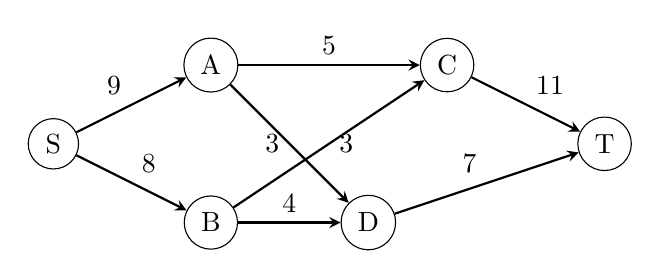
\begin{tikzpicture}
[baseline=(A.base),
 arc/.style={->,thick,>=stealth},
 vertex/.style={draw,circle},]

\node [vertex] at (0cm,0cm) (S) {S};
\node [vertex] at (2cm,1cm) (A) {A};
\node [vertex] at (2cm,-1cm) (B) {B};
\node [vertex] at (5cm,1cm) (C) {C};
\node [vertex] at (4cm,-1cm) (D) {D};
\node [vertex] at (7cm,0cm) (T) {T};

\Arc SA9
\Arc SB8
\Arc AC5
\draw [arc] (A) to node [left, midway] {3} (D);
\draw [arc] (B) to node [right,midway, swap] {3} (C);
\Arc BD4
\Arc CT{11}
\Arc DT7
\end{tikzpicture}

\begin{enumerate}[label=(\alph*)]
\item Find a maximum flow $f$ and all possible minimum cuts.
\item Draw the residual graph $G_f$ (along with its edge capacities), where $f$ is the maximum flow you found in (a). List all the vertices reachable from $S$ and all the vertices from which $T$ is reachable in this residual graph.
\item An edge of a network is called a \emph{critical edge} if increasing its capacity results in an increase in the maximum flow. List all critical edges in the above network.
\end{enumerate}

\q{12}
Suppose you are given a directed graph $G=(V,E)$ with positive integer capacity $c_e$ on each edge $e$, a source $s\in V$ and a sink $t \in V$. You are also given a maximum flow $f$ in $G$. The flow is \emph{acyclic}: there are no cycle in $G$ on which all edges carry positive flow. The flow $f$ is also integer valued.

Now suppose we pick a specific edge $e^* \in E$ and reduce its capacity by 1. Show how to find a maximum flow in the new flow network in time $O(|E|+|V|)$. 

\q{4}{SRTE (Bonus credit)}
Please go to \url{srte.psu.edu} to submit your SRTE feedback (Student Rating of Teaching Effectiveness) which is available after April 17, 2022. This is not required, but if 80\% of you have submitted your evaluations, \emph{all} of you will get this bonus credit. We appreciate your feedback!

\end{qunlist}
\end{document}
